%------------------------------------------%
% Cannabis Data Science
% Date: 12/29/2021
%------------------------------------------%
\documentclass[xcolor={dvipsnames}]{beamer}
\hypersetup{pdfpagemode=FullScreen}
\mode<presentation>{
  \usetheme{Boadilla}
  \usecolortheme{orchid}
  \usefonttheme{default}
  \setbeamertemplate{navigation symbols}{}
  \setbeamertemplate{caption}[numbered]
} 
\usepackage[english]{babel}
\usepackage[utf8x]{inputenc}
\setbeamersize{text margin left=0.5in,text margin right=0.5in}

\usepackage[dvipsnames]{xcolor}
\definecolor{DarkGreen}{RGB}{2, 48, 32}
\definecolor{CalyxGreen}{RGB}{34, 153, 84}
\definecolor{DarkOrange}{RGB}{199, 0, 57}
\definecolor{LightOrange}{RGB}{255, 87, 51}
\definecolor{LightGreen}{RGB}{218, 247, 166}
\definecolor{LightYellow}{RGB}{255, 195, 0}

\setbeamercolor*{palette primary}{bg=LightGreen, fg = DarkGreen}
\setbeamercolor*{palette secondary}{bg=LightGreen, fg=DarkGreen}
\setbeamercolor*{palette tertiary}{bg=LightGreen, fg = DarkGreen}

%------------------------------------------%
% Packages
%------------------------------------------%
\usepackage{amsmath}
\renewcommand*\footnoterule{} %No sperating line on footnote
\usepackage{mathtools} %ANNOTATING EQUATIONS
\usepackage{hhline} %DOUBLBARS
\usepackage[super]{nth}
\usepackage{graphicx, caption, subcaption}

%------------------------------------------%
% Commands
%------------------------------------------%
\newcommand\T{\rule{0pt}{2.5ex}} %TOPSTRUT
\newcommand\B{\rule[-1.25ex]{0pt}{0pt}} %BOTTOMSTRUT
\newenvironment<>{varblock}[2][.9\textwidth] %RESIZED BLOCKS
  {\setlength{\textwidth}{#1}
  \begin{actionenv}#3
    \def\insertblocktitle{#2}\par
    \usebeamertemplate{block begin}}
  {\par\usebeamertemplate{block end}
  \end{actionenv}}
\defbeamertemplate{enumerate item}{largeball} %LARGE BALLS
{\begin{pgfpicture}{-1ex}{-0.65ex}{1.5ex}{1.5ex}
\usebeamercolor[fg]{item projected}
{\pgftransformscale{2.5}\pgftext{\Large\pgfuseshading{bigsphere}}}
{\pgftransformshift{\pgfpoint{0pt}{0.5pt}}
\pgftext{\usebeamerfont*{item projected}\small\insertenumlabel}}
\end{pgfpicture}}
\usepackage{tikz} % FANCY ARROWS
\usepackage{xparse}
\NewDocumentCommand\UpArrow{O{2.0ex} O{black}}{%
   \mathrel{\tikz[baseline] \draw [->, line width=0.5pt, #2] (0,0) -- ++(0,#1);}} % FANCY UPARROW
\NewDocumentCommand\DownArrow{O{2.0ex} O{black}}{%
   \mathrel{\tikz[baseline] \draw [<-, line width=0.5pt, #2] (0,0) -- ++(0,#1);}} % FANCY DOWNARROW
%\vskip 1cm
\makeatletter
\newcommand{\LeftEqNo}{\let\veqno\@@leqno}%LEFT EQUATION #'s
\makeatother

%------------------------------------------%
% Title
%------------------------------------------%
\title[\textbf{Meetup}]{}
\author{Cannabis Data Science}
\institute[]{\Large Meetup}
\date{December \nth{29}, 2021}
\begin{document}
\begin{frame}{}
  
\includegraphics[scale=0.075]{images/logos/cannlytics_logo_with_text_light.png}
  \titlepage
\end{frame}

%------------------------------------------%
% Introduction
%------------------------------------------%
\section{Introduction}

\begin{frame}{}

{\large \textbf{Principles for Data Science}}\vspace{0.5\baselineskip}\\

\vspace{1\baselineskip}

\begin{itemize}

\item \textit{From computer science}- The top 3 rules of programming: reuse, reuse, reuse.

\vspace{1\baselineskip}

\item \textit{From computer science}- Refactor, build-upon, and iterate.

\vspace{1\baselineskip}

\item \textit{From economics}- The choices you make matter.

\vspace{1\baselineskip}

\item \textit{From business} - Take stock of what you already have.

\vspace{1\baselineskip}

\item \textit{From data visualization} - \textbf{SHOW THE DATA}.

\end{itemize}


\end{frame}


%------------------------------------------%
% Promo for Saturday Morning Statistics
%------------------------------------------%
\section{Introduction}

\begin{frame}{}

{\large \textbf{Saturday Morning Statistics}}\vspace{0.5\baselineskip}\\

\vspace{1\baselineskip}

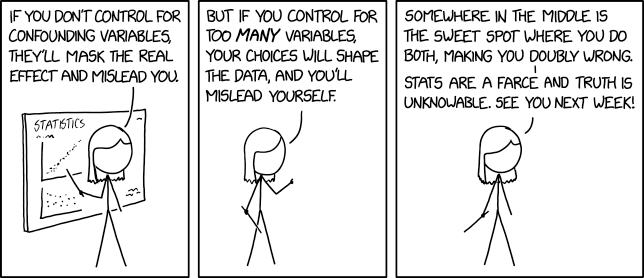
\includegraphics[width=\textwidth]{images/confounding_variables.png}

{\scriptsize Source: https://xkcd.com/2560/}

\vspace{1\baselineskip}

We need a model selection criterion..!

\end{frame}

%------------------------------------------%
% Takeaway
%------------------------------------------%
\section{Conclusion}

\begin{frame}{}

\begin{center}
\begin{minipage}{3.85in}


\includegraphics[width=.25in]{images/prayer.png} {\Large \textbf{Thank you for coming.}}\vspace{0.5\baselineskip}\\

Take some time, discuss any conclusions drawn, and try to analyze some cannabinoids and strains yourself!

\end{minipage}
\end{center}

\end{frame}

%------------------------------------------%
% References
%------------------------------------------%

%\begin{frame}{}
%
%{\large \textbf{References}}\vspace{0.5\baselineskip}\\
%
%{\scriptsize Silvia, J, Iqbal, A, et. al (2014), ‘Economic and Business Forecasting’.}
%
%\end{frame}

\end{document}
